\documentclass{beamer}
    \usetheme{Boadilla}
\usepackage{polyglossia}
    \setmainlanguage{german}
\usepackage{fontspec}
    \setsansfont{Linux Biolinum O}
\usepackage{graphicx}
\usepackage{xcolor}
\usepackage{listings}
    \lstset{language=bash,
	basicstyle=\footnotesize\ttfamily\tiny,
	breaklines=true,
	framextopmargin=50pt,
	frame=bottomline,
	backgroundcolor=\color{white!86!black},
	commentstyle=\color{blue},
	keywordstyle=\color{red},
	stringstyle=\color{orange!80!black}}
\usepackage{amsmath}
\usepackage{amssymb}
\usepackage{siunitx}
\usepackage{booktabs}
\usepackage{float}
\usepackage{tabularx}
\usepackage{caption}
\usepackage{subfig}
\usepackage{tikz}
\usepackage{hyperref}
     \hypersetup{
     colorlinks=true,
     linkcolor=black,
     filecolor=magenta}

\title{\texorpdfstring{\color{blue!50!black}\textbf{Status report - Monday, May 25}}{}}
\subtitle{Programming ideas}
\author{Maurice Donner}
\date{25. May 2020}

\begin{document}

\maketitle

\begin{frame}
\LARGE{Goal:} \normalsize Increase efficiency of scripting\\[0.5cm] \pause
\LARGE{Idea:} \normalsize Instead of reading huge files over and over again,
create multiple threads that read different portions of the file at the same
time.\\[0.5cm]
\begin{minipage}{.3\textwidth}
\begin{figure}[]
    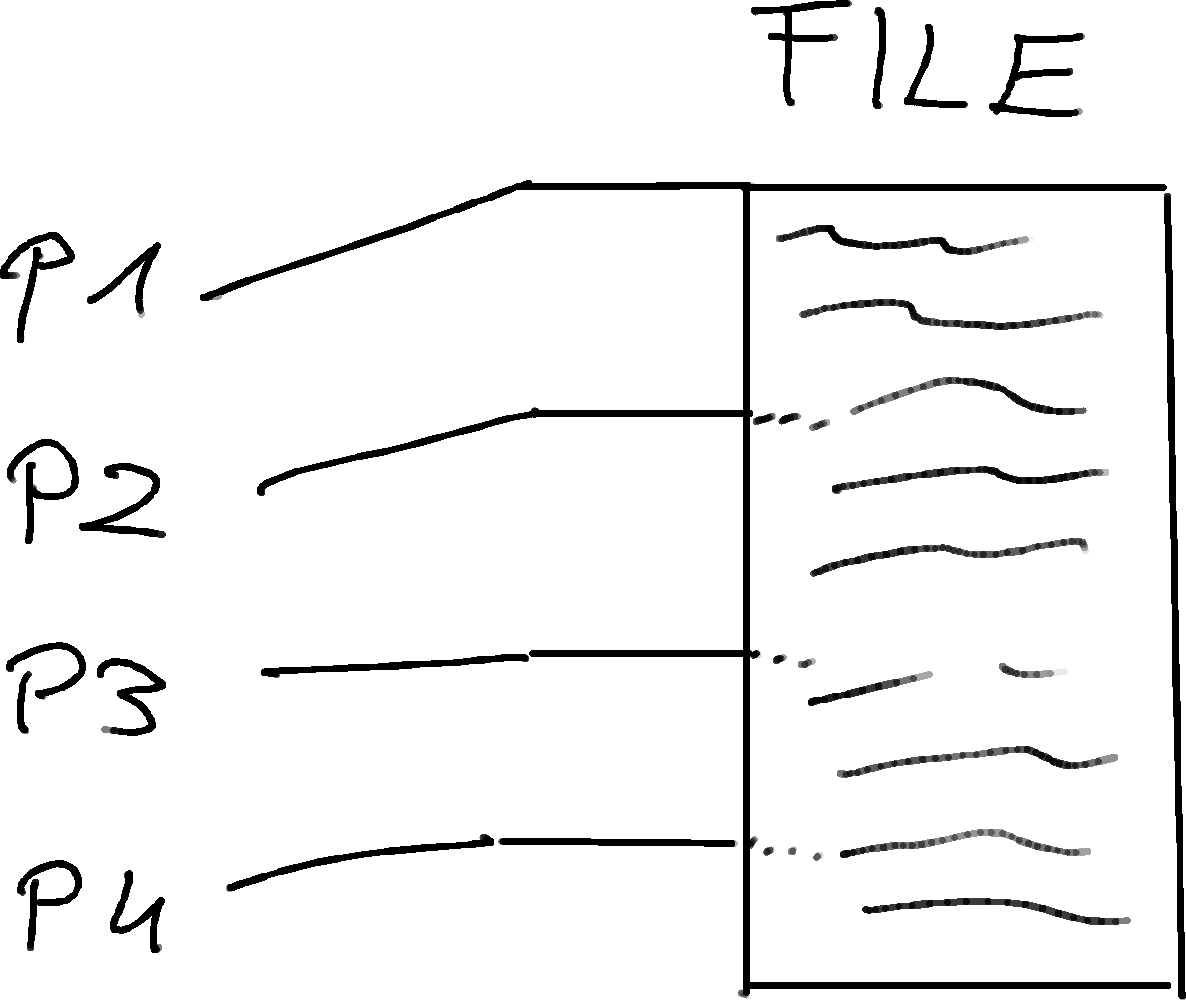
\includegraphics[width=\textwidth]{image.png}
\end{figure}
\end{minipage}
\begin{minipage}{0.05\textwidth}
\ 
\end{minipage}
\pause
\begin{minipage}{0.6\textwidth}
    Advantages: 
    \begin{itemize}
	\item Each PCB has its own seek pointer, that moves over the file
    at different locations. \textbf{In Theory} this should make the entire
    process as fast as opening the file with a text editor. (10+ minutes ->
    10 seconds)
    \item No race conditions, because each process accesses a different portion
    of the file\\[.5cm]
\end{itemize}
\end{minipage}
\pause
BUT: Lots of work for a simple script. String manipulation in c is painful.
\end{frame}
\end{document}
